\emph{Naratologie}, neboli teorie vyprávění, je literární věda, která si během posledních sta let prošla nemalým vývojem. Tématem vyprávěcí teorie se v průběhu dvacátého století zabývali literární teoretici napříč Evropou. Vznikla tedy řada různých typologií a návrhů, jak na téma vypravěče a způsobu vyprávění pohlížet, a jak provádět narativní analýzu.\cite{kubicek-vypravec}

V této kapitole představuji několik základních naratologických pojmů. Dále ukážu vybranou typologii, na níž demonstruji souvislost s touto prací, ????? a zaměřím se na aplikaci vyprávěcí teorie v tvůrčím psaní.

\section{Základy literární teorie a naratologie}

\subsection{Point of view}

Pojem \emph{point of view} lze do češtiny přeložit jako \emph{hledisko}. Hledisko je

TODO najít tu knihu s definicemi pojmů!

\subsection{Formy vyprávění dle osoby}

\emph{Osoba} je mluvnická kategorie sloves v češtině, na základě které se rozlišují základní formy vyprávění. Kromě sloves se tato forma projevuje také v osobních a přivlastňovacích zájmenech.

\paragraph{Ich-forma}

TODO kniha s definicemi

\paragraph{Du-forma}

\paragraph{Er-forma}

\subsection{Systém narativních způsobů}

Z řady narativních typologií jsem se rozhodla vybrat systém, který navrhl jazykovědec a literární teoretik Lubomír Doležel. Doleželův systém vypravěčských způsobů zachycuje stromový graf na obrázku \ref{fig:schema-dolezel}.\cite{dolezel-narativni-zpusoby}

\begin{figure}[ht]
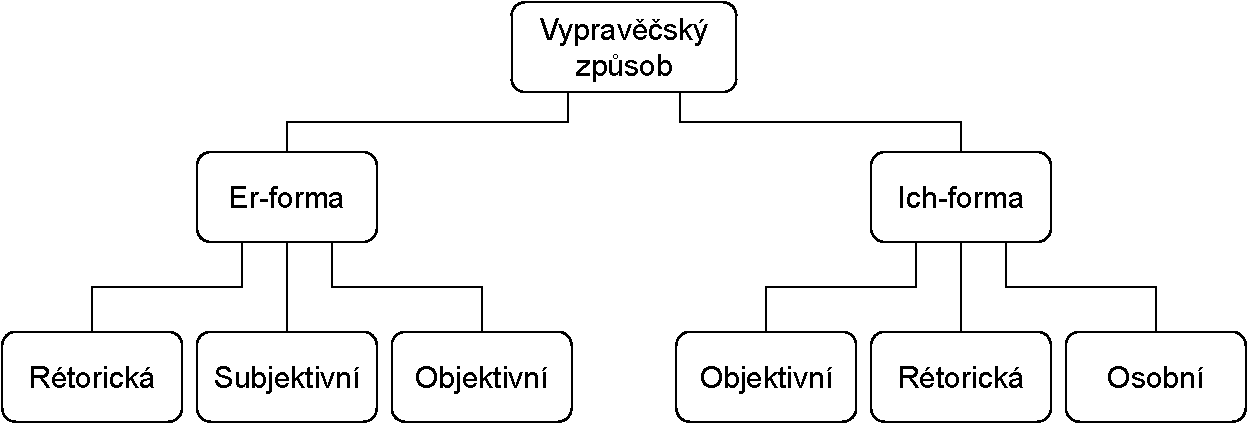
\includegraphics[width=1\textwidth]{data/dolezel-schema.pdf}
\caption{Systém narativních způsobů podle Doležela}
\label{fig:schema-dolezel}
\end{figure}



